\chapter{Conclusion}
\label{chp::conclusion}

\section{Summary and Key Insights}

This dissertation investigates cyber threats to user secrets on the web and proposes methods to defend against them. The work presented in this dissertation makes significant contributions to the field of web security, addressing the increasing threat of cyber crime that hinders the web's function as a key driver of modern communication and commerce. Our dissertation is: \textbf{Password-based authentication protocols should be made obsolete, even though strong, human-chosen, and memorable secrets can be created. This is due to the lack of consensus on password strength and policy, the broader spectrum of threats to such secrets that are not considered in current protocol designs, and usability hurdles like the integration of multi-factor authentication (MFA).} Our contribution is primarily through new data and the proposal (through designs and implementations) of novel schemes. The breadth of this dissertation is substantial and somewhat unusual. However, we believe this holistic approach is important in order to understand the complexity of the systems that guarantee the security of our secrets. To this end, the dissertation is characterised by the journey of user secrets, where each study represents a key point in this journey.

One of our objectives was to empirically analyse data breaches to understand how they occur in the wild and to find opportunities for improvement. We analysed 60 reported data breaches in 2020 and used these insights to lay the foundation for future chapters. We also provide a comprehensive exposition and taxonomy of Man-in-the-Browser malware. This type of malware is fairly easy to develop and is often under-reported, posing a high threat to user secrets. As a result, we further investigate this issue in Chapter~\ref{chp::formless}, where we provide a method that uses an out-of-band device to transmit user secrets with the added advantage of being phishing-resistant. Thus, if the client is compromised, the user's secret will remain safe. We find that the majority of breaches are either due to poor administration by organisations or the exploitation of vulnerabilities in their systems.

In our dissertation, we argue that secure, human-chosen, and memorable secrets can be composed under the right conditions. These conditions, often defined as Password Composition Policies (PCPs), are widely debated, and we showed that most web applications do not follow the standards. To understand what conditions can create such strong passwords, we produced the first human-labelled password dataset. Using this dataset, we demonstrate which empirical passwords can be secure against brute-force and dictionary attacks. PCPs, such as using three random words, are shown to be both secure and usable (i.e., they can be easily communicated and adopted). We also provide a method based on Large Language Models (LLMs) to expedite the labelling process. These models prove to be more accurate and cheaper than their human counterparts for password labelling and decomposition.

Our dataset is also useful for analysing password habits and patterns. It has been well studied that we embed predictable information into our chosen secrets, i.e., passwords. However, limitations in password strength meters, such as \zxcvbn, suggest that we have not fully investigated all the patterns. In Chapter~\ref{chp4::password-composition}, we present a comprehensive set of transformations that can be adopted in password strength meters to better inform users about the security of their passwords. These transformations take into account various linguistic and cultural factors that influence password creation, providing a more accurate assessment of password strength. By incorporating these transformations, password strength meters can offer users more meaningful feedback and encourage the creation of stronger, more resilient passwords.

One way of understanding and improving password strength is through password guessing algorithms. We find that despite the rich body of literature on password guessing, the techniques and algorithms are seldom used in practice, signifying their lack of practicality. We provide a comprehensive exposition of password guessing algorithms in order to address their shortcomings and improve research repeatability.

Finally, in Chapter~\ref{chp::deeid}, we reach the last stop of the secret's journey. Hash functions and key-derivation functions are the security mechanisms at this stage of user secrets. We propose using identity-based cryptosystems that provide a strong form of entity authentication and are zero-knowledge proofs. Using the Fiat--Shamir cryptosystem, we design and implement a scheme. We go on to address ``identity'' on the web. To achieve this, we improve our design and implementation to incorporate blockchain technology, which acts as a decentralised store of identity. We believe this form of identification can transcend human identity and be useful for fictional-entity identity (such as organisations) across the world, as well as machine identity.

Despite showing that human-chosen and memorable secrets can exist, we argue that they are not scalable, and additional security layers merely make password-based authentication systems less usable. These scalability and usability issues highlight the need for a more radical approach to protocol design. WebAuthn and Passkeys are steps in that direction, but the current implementations lack flexibility and raise privacy concerns.

\section{Future Work}

In the process of conducting this research, we experimented with various other ideas that we believe hold value for further exploration.

\subsection{Low-cost EEG-based Authentication}
Continuing the work on password-less authentication (Chapter~\ref{chp::deeid}), we experimented with various other password-less authentication methods, such as EEG-based authentication. Although work has been conducted in this area before, we believe there is a gap in the research---specifically in the EEG hardware itself. The lack of relatively cheap and accurate EEG devices makes this approach highly unreliable and unusable. To address this, we designed a low-cost EEG device based on the OpenBCI system, as shown in Figure~\ref{fig:eeg-device-3d-render}. We used a low-cost and highly available microcontroller---the ESP32. The most important component, the analogue-to-digital converter (ADC), is also the most expensive. We believe that continuing this project would prove highly beneficial for both future researchers and users.

\begin{figure}
    \centering
    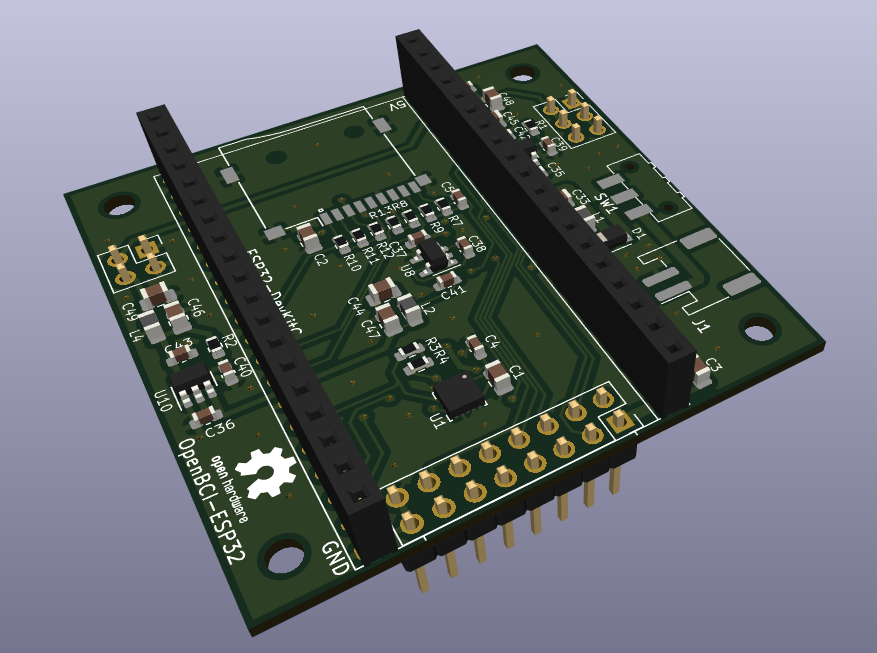
\includegraphics[scale=0.4]{figs/OpenBCI_ESP32_BASE.png}
    \caption{3D render of the AXON EEG device. We designed and manufactured an EEG PCB that uses the ESP32 micro-controller.}
    \label{fig:eeg-device-3d-render}
\end{figure}

\subsection{Credential Stuffing Attack (CSA)}
CSA attacks are often the most silent form of credential theft and account takeovers. Unlike other breaches, most organisations do not suffer the same level of consequences from regulators. Often, organisations may not even be aware that they have suffered a CSA attack. Whilst commercial tools are available to prevent CSA attacks, we believe that further academic research into defending against these attacks would be highly beneficial.

\subsection{Preventing MitB Malware}
In Chapter~\ref{chp3::breaches}, we empirically demonstrated the threat posed by Man-in-the-Browser malware (also known as form grabbers, skimmers, or Magecart-style attacks). Then, in Chapter~\ref{chp::formless}, we designed and implemented a method to circumvent this type of malware. We believe there are ample opportunities for further research on this malware. Little work has been done in creating open-source tools to identify and classify these types of malware.

\subsection{Security-First API Design}
In Chapter~\ref{chp3::breaches}, we found that poor design and human errors could contribute to user secrets being leaked in their millions. An interesting opportunity to mitigate this issue would be to develop necessary tooling that reduces the likelihood of human errors.